\begin{definition}
\emph{(Optimierungsprobleme mit linearen Ungleichungsnebenbedingungen)}
\begin{align}
  \min_{x \in \R^n}\ & f(x)
    \tag{PLU} \label{prob:opt_prob_mit_lin_ungl_nebenbed} \\
                 \nb & Ax = b \notag \\
                     & Gx \leq r \notag
\end{align}
$A$ sei eine $(m \times n)$-Matrix mit $m \leq n$ und $b \in \R^m$.
$G$ sei eine $(p \times n)$-Matrix und $r \in \R^p$.
\end{definition}

D.\,h., die Menge $\F$ sieht hier so aus:
$\F = \{ x \in \R^n\ |\ A x = b,\ G x \leq r \}$.

Seien $a_k \in \R^n$, $k = 1,\ldots,m$, bzw. $g_j \in \R^n$, $j = 1,\ldots,p$,
Vektoren in der Matrix $A$ bzw. $G$, sodass
\begin{equation}
\label{eq:zerlegung_von_A_und_G}
  A =
  \left(
    \begin{array}{c}
      a_1^T \\
      \vdots \\
      a_m^T
    \end{array}
  \right)
\quad \text{und} \quad
  G =
  \left(
    \begin{array}{c}
      g_1^T \\
      \vdots \\
      g_p^T
    \end{array}
  \right).
\end{equation}

Seien $b_k \in \R$, $k = 1,\ldots,m$, bzw. $r_j \in \R$, $j = 1,\ldots,p$,
die Elemente von $b$ bzw. $r$.
Dann k�nnen wir das Problem~\eqref{prob:opt_prob_mit_lin_ungl_nebenbed}
wie folgt ausf�hrlicher schreiben.
\begin{align*}
  \min_{x \in \R^n}\ & f(x) \\
     \nb & \langle a_k, x \rangle = b_k \text{ f�r } k = 1,\ldots,m \\
         & \langle g_j, x \rangle \leq r_j \text{ f�r } j = 1,\ldots,p
\end{align*}

\begin{example}\label{example:opt_prob_mit_lin_ungl_nebenbed}
\emph{(Vgl. Beispiel 16.4 in \cite[S.~475]{nocedal})}\\
Ein einfaches zweidimensionales Beispiel
eines Optimierungsproblems~\eqref{prob:opt_prob_mit_lin_ungl_nebenbed}
ist
\begin{equation}
\begin{split}
\min_{x\in\R^2}\ (x_1 - 1)^2 + (x_2 & - 2.5)^2 \\
\nb -x_1 + 2 x_2 & \leq 2 \\
x_1 + 2 x_2 & \leq 6 \\
x_1 - 2 x_2 & \leq 2 \\
x_1, x_2 & \geq 0. \\
\end{split}
\end{equation}
Die Abbildung~\ref{fig:beispiel_opt_prob_mit_lin_ungl_nebenbed}
zeigt die zul�ssige Menge $\F$,
die H�henlinien der Zielfunktion und
die optimale L�sung~$\xopt$.
\end{example}

\begin{figure}[h]
\centering
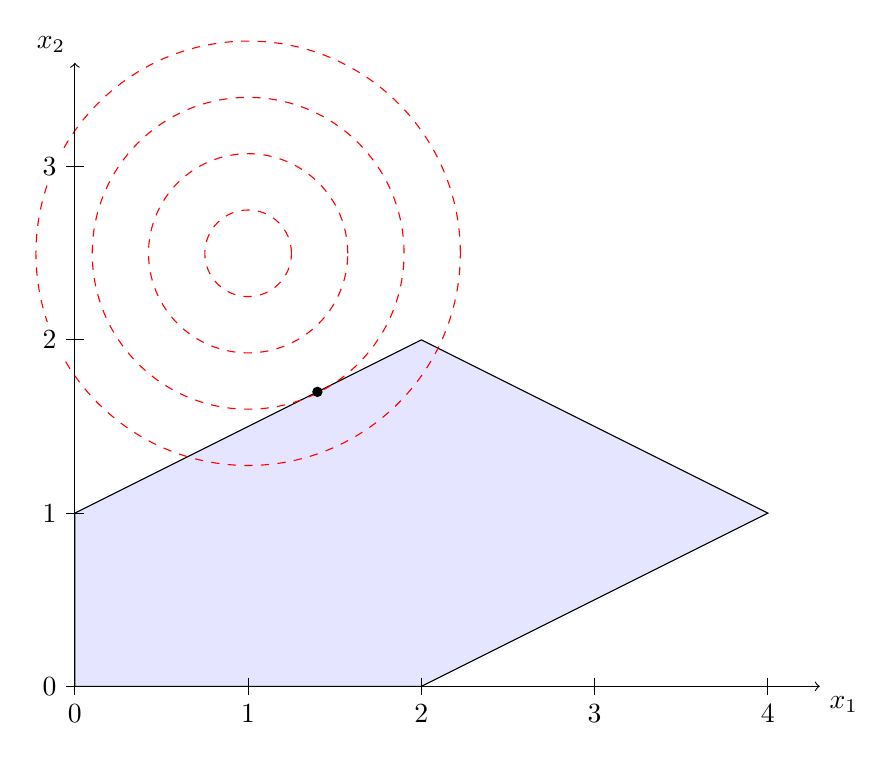
\begin{tikzpicture}[scale=2.2]
  % Schreibe x*
  \draw (1.4,1.7) node[above,fill=white] {$\xopt$};
  % Die zul�ssige Menge
  \draw[fill=blue!10] (0,0) -- (0,1) -- (2,2) -- (4,1) -- (2,0) -- cycle;
  \draw (1.7,1) node {$\F$};
  % Die Niveaulinien
  \foreach \r in {0.25, 0.575, 0.9, 1.225}
    \draw[dashed,color=red] (1,2.5) circle (\r);
  % Koordinatenachsen
  \draw[->] (0,0) -- (4.3,0) node [below right] {$x_1$};
  \foreach \x in {0,...,4}
    \draw (\x,0.05) -- (\x,-0.05) node [below] {\x};
  \draw[->] (0,0) -- (0,3.6) node [above left] {$x_2$};
  \foreach \y in {0,...,3}
    \draw (0.05,\y) -- (-0.05,\y) node [left,fill=white] {\y};
  % Der Kreis f�r x*
  \fill (1.4,1.7) circle (0.03);
\end{tikzpicture}
\caption{Geometrische Darstellung
des Beispiels~\ref{example:opt_prob_mit_lin_ungl_nebenbed}}
\label{fig:beispiel_opt_prob_mit_lin_ungl_nebenbed}
\end{figure}

\begin{example}\label{example:abstand_zw_dreiecken_problem}
\emph{(Vgl. Beispiel 13.2 in \cite[S.~415f]{antoniou})}\\
Gegeben seien zwei Dreiecke $R$ und $S$
in der Abbildung~\ref{fig:abstand_zw_dreiecken}.
Gesucht ist der k�rzeste Abstand zwischen diesen Dreiecken
und die zugeh�rigen Punkte $r^* \in R$ und $s^* \in S$, die
diesen k�rzesten Abstand bilden.

\begin{figure}[h]
\centering
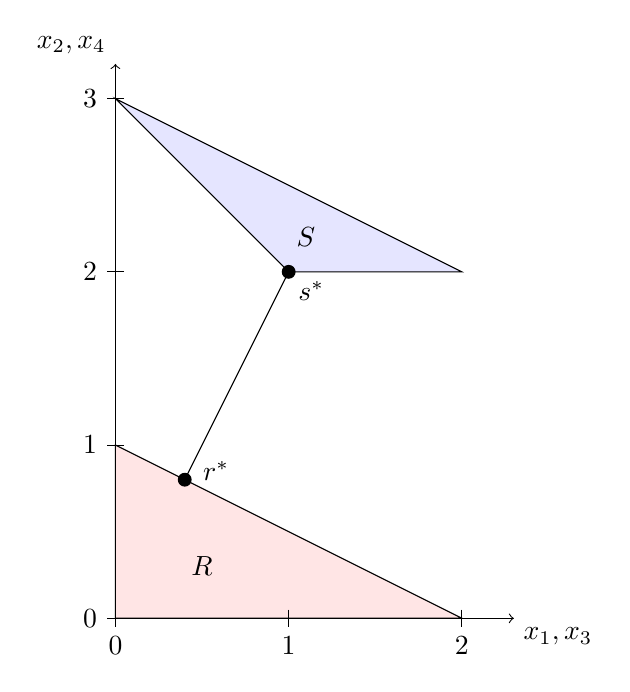
\begin{tikzpicture}[scale=2.2]
  % Dreieck R
  \draw[fill=red!10] (0,0) -- (0,1) -- (2,0) -- cycle;
  \draw (0.5,0.3) node {$R$};
  % Dreieck S
  \draw[fill=blue!10] (0,3) -- (1,2) -- (2,2) -- cycle;
  \draw (1.1,2.2) node {$S$};
  % Punkt r*
  \fill (0.4,0.8) circle (0.04);
  \draw (0.45,0.85) node [right] {$r^*$};
  % Punkt s*
  \fill (1,2) circle (0.04);
  \draw (1,2) node [below right] {$s^*$};
  % Linie zwischen r* und s*
  \draw (0.4,0.8) -- (1,2);
  % Koordinatenachsen
  \draw[->] (0,0) -- (2.3,0) node [below right] {$x_1, x_3$};
  \foreach \x in {0,...,2}
    \draw (\x,0.05) -- (\x,-0.05) node [below] {\x};
  \draw[->] (0,0) -- (0,3.2) node [above left] {$x_2, x_4$};
  \foreach \y in {0,...,3}
    \draw (0.05,\y) -- (-0.05,\y) node [left] {\y};
\end{tikzpicture}
\caption{Geometrische Darstellung
des Beispiels~\ref{example:abstand_zw_dreiecken_problem}}
\label{fig:abstand_zw_dreiecken}
\end{figure}

Seien $r = (x_1, x_2)^T \in R$ und $s = (x_3, x_4)^T \in S$.
Der quadratische Abstand zwischen $r$ und $s$ ist durch
\begin{equation}
  \| r - s \|^2 = (x_1 - x_3)^2 + (x_2 - x_4)^2 = x^T H x
\end{equation}
gegeben, wobei
\begin{equation}
  H :=
  \left(\begin{array}{cccc}
     1 &  0 & -1 &  0 \\
     0 &  1 &  0 & -1 \\
    -1 &  0 &  1 &  0 \\
     0 & -1 &  0 &  1
  \end{array}\right).
\end{equation}

Die Bedingungen $r \in R$ und $s \in S$ sind durch die Ungleichungen
\begin{equation}
\begin{split}
    x_1, x_2 & \geq 0 \\
  x_1 + 2x_2 & \leq 2 \\
         x_4 & \geq 2 \\
   x_3 + x_4 & \geq 3 \\
  x_3 + 2x_4 & \leq 6
\end{split}
\end{equation}
gegeben.
D.\,h., das Problem kann als Optimierungsproblem mit einer quadratischen
Zielfunktion und linearen Ungleichungsnebenbedingungen dargestellt werden.
\end{example}

Der folgende Satz hat sich als besonders hilfreich erwiesen,
um eine lokale L�sung
des Problems~\eqref{prob:opt_prob_mit_lin_ungl_nebenbed}
zu charakterisieren.

\begin{theorem} \label{satz:karush_kuhn_tucker}
\emph{(Karush-Kuhn-Tucker-Satz, vgl. Satz 5.4.7 in \cite[S.~193]{alt})}\\
Sei $\xopt$ lokale L�sung des Problems~\eqref{prob:opt_prob_mit_lin_ungl_nebenbed} und
$f$ sei in~$\xopt$ differenzierbar.
Dann existieren die Vektoren $\lambda \in \R^m$ und $\mu \in \R^p$
zu~$\xopt$ mit
\begin{align}
   \nabla f(\xopt) + A^T \lambda + G^T \mu & = 0 \\
  \mu_j (\langle g_j,\xopt \rangle - r_j ) & = 0 \text{ f�r } j = 1,\ldots,p \\
                                       \mu & \geq 0
\end{align}
Die Vektoren $\lambda$ und $\mu$ hei�en Lagrange-Multiplikatoren zu $\xopt$.
\end{theorem}

Sei $x \in \F$. Wir bezeichnen mit
\begin{equation}
\label{eq:indexmenge_der_aktiven_restr}
  J(x) := \{ 1 \leq j \leq p \ | \ \langle g_j,x \rangle = r_j \}
\end{equation}
die Indexmenge der in $x$ aktiven Ungleichungsrestriktionen.

\begin{theorem}
\label{satz:hinr_bed_fuer_prob_mit_lin_ungl_nebenbed}
\emph{(Hinreichende Optimalit�tsbedingung, vgl. Satz 5.4.13 in
\cite[S.~198]{alt})}\\
Sei $f$ in $\xopt \in \F$ zweimal stetig differenzierbar. Die notwendigen
Bedingungen von Satz~\ref{satz:karush_kuhn_tucker} seien erf�llt
und es gelte mit $\alpha > 0$
\begin{equation}
d^T f''(\xopt) d \geq \alpha \|d\|^2 \quad
  \forall d \in \R^n :
  \begin{cases}
    Ad = 0, & \\
    \langle g_j,d \rangle \leq 0
      & \text{f�r } j \in J(\xopt) \text{ mit } \mu_j = 0, \\
    \langle g_j,d \rangle = 0
      & \text{f�r } j \in J(\xopt) \text{ mit } \mu_j > 0.
  \end{cases}
\end{equation}
Dann ist $\xopt$ eine strikte lokale L�sung des
Problems~\eqref{prob:opt_prob_mit_lin_ungl_nebenbed}.
\end{theorem}

Ein Spezialfall des Problems~\eqref{prob:opt_prob_mit_lin_ungl_nebenbed} ist das
Optimierungsproblem mit unteren und oberen Schranken f�r die Variablen.

\begin{definition}
\emph{(Optimierungsprobleme mit Variablenbeschr�nkungen)}
\begin{align}
  \min_{x \in \R^n}\ & f(x) \tag{PVB} \label{prob:opt_prob_mit_var_beschr} \\
                 \nb & a \leq x \leq b \notag
\end{align}
$a, b \in \R^n$ mit $a \leq b$.
\end{definition}

Die Nebenbedingung ist
�quivalent zu
$G x \leq r$
mit
$G := \left( \begin{array}{c} -I_n \\ I_n \end{array} \right)$ und
$r := \left( \begin{array}{c} -a \\ b \end{array} \right)$.

% TODO: sufficient condition?
